\chapter{Global System for Mobile Communications}
This chapter describes the fundamental parts of \gls{GSM} with prime
focus on explaining communication over the Um interface, which we will
look closer at in \cref{sec:gsm_air_interface}. The infrastructure of
\gls{GSM} is usually pictured as a tree as shown in
\cref{fig:gsm_infrastructure} where the \gls{MSC}, with connection to
the \gls{PSTN}, is the trunk and the \glspl{BSC}, and \glspl{BTS},
make branches. The \gls{MSC} is a backhaul part of the core of GSM
known as the \gls{NSS}, which links to the \gls{PSTN} and serves
functionality such as mobile registration, mobility management, call
control and more.

\begin{figure}[H]
  \centering
  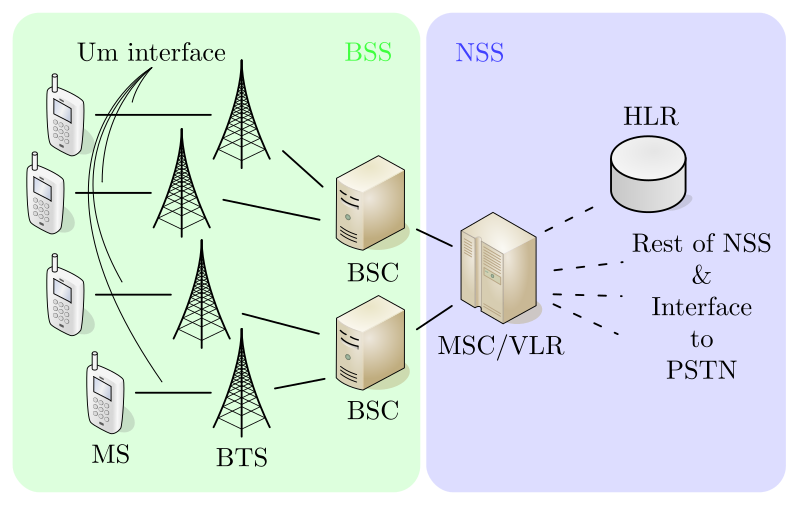
\includegraphics[width=0.75\textwidth]{figures/gsm_infrastructure}
  \caption{The infrastructure of the outermost part of \gls{GSM}
    combined by the BSS and NSS with \glsentryfullpl{MS},
    connected to the \glspl{BTS}~\cite[p. 11, 21--44]{gsmtolte}.}
  \label{fig:gsm_infrastructure}
\end{figure}

The \gls{HLR}, and \gls{VLR}, are databases storing records of
authenticated subscribers e.g.\ mobile phones where the \gls{HLR}
stores each subscriber and \gls{VLR} stores only subscribers in
coverage of the corresponding \gls{MSC}.\ When a subscriber moves into
a different coverage area, the new \gls{MSC} in this area fetches the
record from the \gls{HLR} and stores it locally in its \gls{VLR}.\ The
record in the old \gls{MSC} is then deleted, and by storing these
records locally in the \gls{VLR}, the load is reduced on the shared
\gls{HLR} database~\cite[p. 13-17]{gsmtolte}. Subscriber registration
and mobility management is done by the \gls{MSC} which also handles
call establishment and call routing between two
users~\cite[p. 11-13]{gsmtolte} and by digging further into the
\gls{BSS}, there is the \gls{BSC} that controls medium allocation on
the Um interface, smooth handover to a different base station while
roaming, time advance in transmission and signal power control and
thus by combining these two entities a link between two subscribers
can be established and maintained~\cite[p. 30-34]{gsmtolte}. A
\gls{BSC} controls a set of \glspl{BTS} which are directly linked to
the Um interface.

\section{Base Transceiver Station}
The \gls{BTS}, links directly to the Um interface and it ensures a
radio link from the mobile phone to the backhaul network. The
\gls{BTS} covers an area wirelessly known as a cell in which mobile
devices must remain to ensure coverage and access to mobile
services. As stated above, the \gls{BSC} enables extra flexibility and
hands over mobile devices to a different BTS if one were to move out
of coverage, however, this means that the new area must be covered by
another BTS.\ By measuring signal strength, the \gls{BSC} can
determine when the best time is to perform a handover to a different
\gls{BTS}.\

\begin{figure}[H]
  \centering
  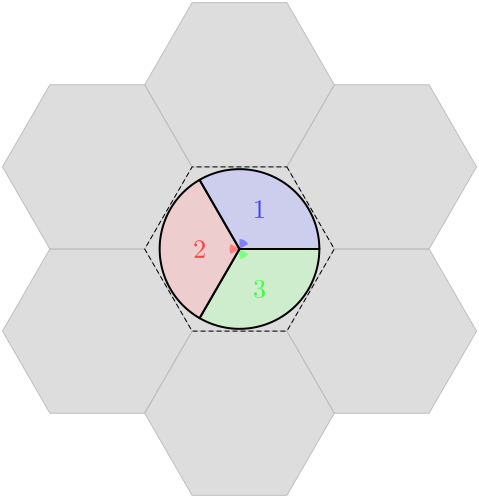
\includegraphics[width=0.4\textwidth]{figures/gsm_cell}
  \caption{A \gls{GSM} cell sectorized into three areas that make a
    part of a cellular structure.}
  \label{fig:gsm_cell}
\end{figure}

\gls{BTS}s are positioned such that they cover a sector within a cell,
commonly these sectors make a $120^{\circ}$ degree angle thus a cell
is divided into two or three sectors as seen in \cref{fig:gsm_cell},
and to avoid interference, each sector operates at different
frequencies. Dividing a cell into three sectors enables a better reuse
of frequencies without interferring with neighbor sectors. These areas
vary much in size because capacity is limited, but generally they can
vary from $35km$ down to $100m$ in distance. $35km$ is only
theoretical and due to the required signal power these areas are much
smaller in practice, $3$ to $4km$ is common in residential and
business areas~\cite[p. 23]{gsmtolte}.

\section{Um air interface}
\label{sec:gsm_air_interface}
Within a sector, the \gls{BTS} transmits in a frequency spectrum
licensed to commercial operators and depending on what country, these
spectra differs. The \gls{GSM} standard specifies a couple of
different frequency bands; e.g. $850\si{MHz}$, $900\si{MHz}$ primary,
$900\si{MHz}$ extended, $900\si{MHz}$ railway-specific, $1800\si{MHz}$
and $1900\si{MHz}$. In Denmark, $900\si{MHz}$ and $1800\si{MHz}$ are
reserved for GSM~\cite{frequencyspectrum}. In each of these bands
there are channels with a width of $200\si{kHz}$ that can be assigned
to a specific sector. For example, this leaves $124$ channels in the
$900\si{MHz}$ band and each of these channels are identified by a
number, the \gls{ARFCN}~\cite[p. 21--22]{gsmtolte}. The channel number
can be calculated to- and from the corresponding carrier frequency for
$900\si{MHz}$ primary with the equations given in
\cref{eq:arfcn}~\cite[p. 10]{arfcn}.

\begin{equation}
  \begin{aligned}
    f_{ul} &= 900\si{MHz} + 0.2\si{MHz} \cdot n & \quad \text{for } 1 \leq n \leq 124\\
    f_{dl} &= f_{ul} + 45\si{MHz} &
  \end{aligned}
  \label{eq:arfcn}
\end{equation}

$f_{ul}$ and $f_{dl}$ refer to carrier frequencies for uplink and
downlink, respectively, in a given channel $n$. The equation is
similar for other frequency bands where $900\si{MHz}$ in the equation
refers to the band, $0.2\si{MHz}$ remains the same for all bands, but
$n$ may need to be offset in certain cases and \gls{ARFCN}, values are
abnormal thus different in all bands. The $45\si{MHz}$ offset for the
downlink expression vary with the number of channels in a specific
band. The specifics are defined in the standard~\cite[p. 10]{arfcn}.
\subsection{Multiplexing}
As just introduced, \gls{GSM} defines a set of channels given by the
\gls{ARFCN} number, each of these numbers correspond to a carrier
frequency with a bandwidth of $200\si{kHz}$. A \gls{BTS} may
communicate with multiple users either at different frequencies or by
taking turn rapidly for each user. The first method is called
\gls{FDMA}, which is described briefly next and the other method is
called \gls{TDMA}.\

\subsubsection{Frequency Division Multiple Access}
Given the $124$ channels in the $900\si{MHz}$ frequency band, a
\gls{BTS} is not limited to just three channels for each of its
sectors. By installing multiple \glspl{TRX}, a single sector can serve
an increased number of users at the same time and each of these
\glspl{TRX} operate at a uniquely assigned frequency within the
band. Communication is thus multiplexed using \gls{FDMA} both within a
single sector and across the whole cell.

\subsubsection{Time Division Multiple Access}
Apart from frequency multiplexing, \gls{GSM} also divides
communication in time. Such a division results in a \gls{TDMA} frame
that consists of eight timeslots each of which can transfer a
so-called burst with a duration of $577\si{\mu s}$.
\cref{fig:tdma_frame} shows the structure of a \gls{TDMA} frame with
two timeslots carrying data. Timeslot $0$ and $1$ on the main
frequency is mostly used for \gls{BTS} signalling and by listening to
this timeslot a mobile device can determine if the corresponding
frequency is currently used by a \gls{BTS}.\

\begin{figure}[H]
  \centering
  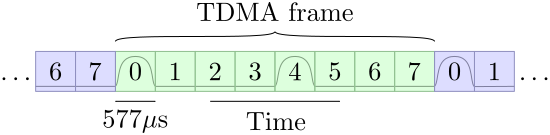
\includegraphics[width=0.6\textwidth]{figures/tdma_frame}
  \caption{A TDMA frame consisting of eight timeslots numbered from
    $0$ to $7$ with timeslot $0$ and $4$ carrying a burst.}
  \label{fig:tdma_frame}
\end{figure}

A subscriber is allocated a single timeslot in the up- and downlink
and it is only allowed to send at that point in time. Such a timeslot
allocation can be thought as a physical channel. Transmission and
reception therefore occurs at an interval of $4.6\si{ms}$, the width
of a \gls{TDMA} frame.

The information carried in each burst depends on what type of
information is transmitted. The burst bit configuration differs for
broadcast signals, traffic communication and direct signalling to
mobile devices. The different types of bit configurations are; a
normal burst, frequency correction, synchronization, dummy and an
access burst as seen in \cref{fig:burst}. The normal burst is used for
voice traffic, both transmission and reception and it carries
encrypted sectionized bits in a pair. Inbetween this pair, a training
sequence bit pattern is transmitted to compensate for interference
caused. Two stealing bits are transmitted before and after the
training sequence and they are used to indicate if either of the
sections of encrypted bits are stolen for urgent signalling. At the
beginning and end of a burst, a pattern of bits, tail bits, are
transmitted to help detect these transitions and before and after
these patterns a brief guard time period is present to avoid
overlapping of neighbor timeslots. The frequency correction burst is
transmitted by the \gls{BTS} and is used by the mobile device to
synchronize its local oscillator to the clock frequency of the
\gls{BTS}.\ The \gls{BTS} also transmits a synchronization burst which
is used to time synchronize to a \gls{TDMA} frame number (see
\cref{sec:2651multiframe}). A dummy burst is transmitted in all
timeslots by the \gls{BTS} if they aren't already occupied and it is
used to measure signal strength at the receiver which then transmits
the result back to the \gls{BTS} and the \gls{BSC}.\ The \gls{BSC}
then determines if a handover would be sufficient. The access burst is
used to correctly control burst timing for extra ensurance of
collision-free bursts. Timing advance depends on the distance between
the subscriber and the \gls{BTS} thus this must be adjusted for bursts
to arrive at either end at the right moment in
time~\cite[p. 25--26]{gsmtolte}.

\begin{figure}[H]
  \centering
  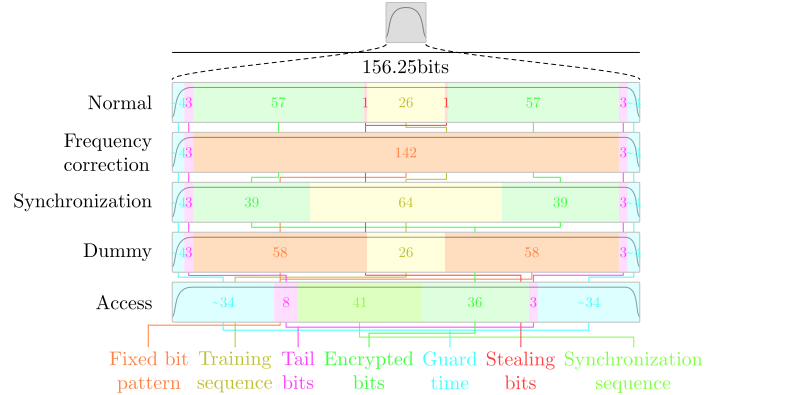
\includegraphics[width=\textwidth]{figures/burst}
  \caption{Five different types of \gls{GSM} bursts each with a
    different bit configuration~\cite[p. 19--31]{bursts}.}
  \label{fig:burst}
\end{figure}

All these timeslots, or physical channels as they can also be thought
as, are arranged into logical channels, which accomplish some of the
functions as mentioned above for each type of burst. Not all data is
necessary to transmit every TDMA frame, say a frequency correction
burst or a synchronization burst thus these types of different data
are transmitted at a greater interval. Depending on whether this data
is a broadcast message, some exchanged information to an idle mobile
device or a speech channel, the interval can vary differently. The
\gls{GSM} standard defines two types of groups of \gls{TDMA} frames
for this purpose, the $26$ multiframe and the $51$ multiframe. These
two groups of frames are repeated infinitely and their content is
described below~\cite[p. 27]{gsmtolte}.

\subsection{26- and 51 multiframe}
\label{sec:2651multiframe}
The synchronization burst enables synchronization to a specific
\gls{TDMA} frame number which is the number of a \gls{TDMA} frame in
either the 26 frame or the 51 frame. The synchronization burst is
repeated every tenth \gls{TDMA} frame in timeslot $0$ on the main
carrier frequency and is part of the 51 frame. The synchronization
burst is mapped onto the logical \gls{SCH}, which makes five timeslots
out of $51$. Apart from the \gls{SCH}, frequency correction also takes
place in the $51$ frame together with \gls{BTS} broadcast information,
paging of a mobile device, timeslot allocation etc.\ and all these are
mapped in a specific order and to a specific frame number in the $51$
frame.

\begin{figure}[H]
  \centering
  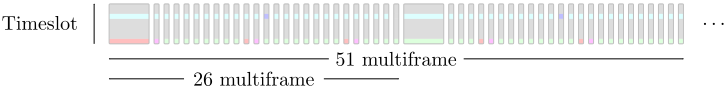
\includegraphics[width=\textwidth]{figures/2651frame}
  \caption{A bundle of frames represented as the $26$- and $51$
    multiframe where light blue color represents subscriber traffic,
    dark blue represents signal measurements, red represents frequency
    correction, purple represents synchronization and the light green
    represents other types of information such as paging information,
    location updates, timeslot allocation requests etc.}
  \label{fig:2651frame}
\end{figure}

The $26$ frame is used for traffic and the timeslot allocation remains
to an interval of one \gls{TDMA} frame until the timeslot in frame number
$12$ which, instead of data, is used to transmit signal quality
measurements and timing advance control information. For both the
$26$- and $51$ frame some frames are idle and no information is
transfered in this time period. Frame number $25$ is idle in the 26
frame thus an on-going call suffers two very brief moments of
interruptions twice in every $26$ frame, but the interruptions are not
audible to the user. Similar situations occur in the $51$ multiframe
as seen on \cref{fig:2651frame}~\cite[p. 26--28]{gsmtolte}. These
categorizations of channels are explained next.

\subsection{Channels}
As with the \gls{SCH}, other types of information are mapped onto a
logical channel. The logical signalling channels are described as
follows\cite[p. 26--29]{gsmtolte}:
\begin{itemize}
\item \textbf{FCCH}: The frequency correction burst is transmitted
  every tenth \gls{TDMA} frame on timeslot $0$ called \gls{FCCH} and
  is used by the mobile device to detect and correctly tune in to the
  frequency of the \gls{BTS}.\ Its local oscillator becomes
  synchronized with the \gls{BTS} clock frequency by searching for a
  unmodulated sine wave carrier at an offset of
  $67.7\si{kHz}$~\cite{bursts}.

\item \textbf{SCH}: During synchronization, synchronization bursts on
  the \gls{SCH} channel are used to identify the \gls{BTS} and
  synchronize to its \gls{TDMA} frame clock frequency.

\item \textbf{BCCH}: The \gls{BCCH}, carries the main information
  about the current cell and neighbor cells and mobile devices monitor
  this channel while idle.

\item \textbf{RACH}: \Gls{RACH} is a common
  channel used by all mobile devices for requests of mobile originated
  calls and sending and fetching of \gls{SMS}, messages.

\item \textbf{AGCH}: During call establishment, the mobile device must
  request a channel which the \gls{BTS} grants access to by either
  allocating a \gls{SDCCH}, or in exceptional cases, a \gls{TCH}.\ The
  \gls{AGCH}, is used for this purpose and is carried by the \gls{RACH}.\

\item \textbf{PCH}: When an incoming call is attempted, mobile devices
  are paged on the \gls{PCH}, in the location area on all \glspl{BTS}
  belonging to the \gls{BSC} controlling this area. The mobile device
  is aware of its own identity and the paging message contains the
  specific mobile device's identity thus all devices know if the
  paging message belong to them individually.

\item \textbf{SDCCH}: The dedicated control channel is a pure
  signalling channel used during call establishment before being
  assigned a \gls{TCH}, transmission and reception of \gls{SMS}
  messages and location area update procedures.

\item \textbf{SACCH}: The \gls{SACCH}, is used to transmit radio
  signal measurements and timing advance in the $26$ frame as
  mentioned above. The network may perform handovers to other cells
  based on the mobile device's feedback if necessary.

\item \textbf{FACCH}: In contrast to \gls{SACCH}, this channel is a
  fast alternative, used in urgent signalling and it steals a data
  section in a normal burst. The abbreviation comes from \gls{FACCH}.
\end{itemize}

All these different channels are further categorized into one of two
types, a broadcast, a \gls{CCCH} or a \gls{DCCH}. Thus, a channel can
either be dedicated to one user or be broadcast to a common group of
users. In this sense, a broadcast- and a common channel are similar.

\subsection{Channel coding}
\label{sec:channel_coding}
Since the air interface is prone to transmission errors because of
sudden frequent changes in the radio environment, some steps are taken
to counter these errors, namely the methods: block coding, convolution
coding and interleaving, in hope for a successful recreation of data
due to lost bits.

\subsubsection{Block coding}
The block coding part, e.g.\ for speech frames, extracts a sequence of
$260$ bits into two chunks referred to as class $1$, $182$ bits, and
class $2$, $78$. The prior chunk is further split into two subclasses
$1a$ of $50$ bits and $1b$ of $132$ bits. The $1a$ subclass adds three
bits of \gls{CRC}, and this new chunk is concatenated with $1b$ and
four filler bits. The concatenation is then protected by the
convolutional code and the result is prepended with the unprotected
chunk, class $2$. The filler bits appended to class $1b$ ensures the
final size of the convolved bits to fit in four bursts, $456$
bits~\cite[p. 17]{coding}. Frames sent on broadcast channels are convolved
for the whole sequence of bits. Their input is $184$ bits and a
\gls{CRC} parity check of $40$ bits and $4$ filler bits are
added. After convolution, the final size is also stretched over four
bursts.

\subsubsection{Convolution coding}
The class $1$ data is convolved with a convolution code with a code
rate of $1/2$ such that two coded bits correspond to a single bit of
data. Lowering the code rate gives better correction potential in turn
for less actual data being sent. \gls{GSM} specifies eight different
polynomials used for convolving the data bits. For the full-rate
\gls{TCH}, data bits at index $i$ are convolved using the two
polynomials
\begin{equation}
  \begin{aligned}
    C_0\para{D} &= 1 + D^3 + D^4\\
                &\Downarrow\\
    C_0\para{D_i} &= D_i + D_{i - 3} + D_{i - 4} \mod 2,\\
    & \qquad \text{and}\\
    C_1\para{D} &= 1 + D + D^3 + D^4\\
                &\Downarrow\\
    C_1\para{D_i} &= D_i + D_{i - 1} + D_{i - 3} + D_{i - 4} \mod 2.
  \end{aligned}
\end{equation}
A sequence of encoded bits are then made of code words $W_c =
\para{C_0, C_1}$ where each word represents a single data bit. To
decode this again, a common way is to perform the Viterbi algorithm
based on the Hamming distance as path metrics.

\subsubsection{Viterbi algorithm}
The Viterbi algorithm is an algorithm to find the most likely sequence
of hidden states. In the case of decoding, the hidden states are data
bits that are derived from the code words, $W_c$. The number of states
correspond to $2^{\abs{W_c}}$ where each state represent the bit
pattern of a code word. \cref{fig:viterbi_fsm} illustrates possible
transition decisions and the Hamming distance is used to calculate the
branch metric. The Hamming distance is the number of changing bits of
the input compared to the possible transitions in each state. For
example, starting in state $S_0$ with an input of a $\para{1,1}$ code
word, the goal is to minimize the total Hamming distance from $t_0$ to
$t_n$, where $t_n$ is the time of the last data bit. The smallest
metric from $t_0$ to $t_1$ is zero since there are no bits that differ
between the code word $\para{1,1}$ and the $\para{1, 1}$
transition. In contrast, the code word, $\para{1,1}$, has a metric
distance to $\para{0, 0}$ of length
two~\cite[p. 235--239]{principledigcom}.

\cref{fig:viterbi_trellis} illustrates the finite state machine of
\cref{fig:viterbi_fsm} over time. For each change of state, a binary
decision is made and once the algorithm terminates, the state tree is
traced back and the binary sequence with the smallest total metric
from $t_0$ to $t_n$ is the estimated decoded data.

\begin{figure}[H]
  \centering
  \begin{tikzpicture}[>=stealth',shorten >=2pt,auto,node distance=3cm]
    \node[initial,state] (S_0)                {$S_0$};
    \node[state]         (S_1) [right of=S_0] {$S_1$};
    \node[state]         (S_2) [below of=S_0] {$S_2$};
    \node[state]         (S_3) [below of=S_1] {$S_3$};

    \path[->]
      (S_0) edge [loop above,
                  dashed]     node {$\para{0,0}$} (S_0)
            edge [bend left]  node {$\para{1,1}$} (S_1)
      (S_1) edge [bend right,
                  dashed]     node [above left] {$\para{1,0}$} (S_2)
            edge [bend left]  node {$\para{0,1}$} (S_3)
      (S_2) edge [bend left,
                  dashed]     node {$\para{1,1}$} (S_0)
            edge [bend right] node [below right]{$\para{0,0}$} (S_1)
      (S_3) edge [bend left,
                  dashed]     node {$\para{0,1}$} (S_2)
            edge [loop below] node {$\para{1,0}$} (S_3);
  \end{tikzpicture}
  \caption{A \glsentryfull{FSM}, of the Viterbi decode algorithm. The look of
    line transitions determine the output where dashed lines represent
    an output of $0$ and normal lines an output of $1$ at time $t$.}
  \label{fig:viterbi_fsm}
\end{figure}

\begin{figure}[H]
  \centering
  \begin{tikzpicture}[>=stealth',shorten >=2pt,auto]
    \foreach \i in {1,...,4} {
      \pgfmathtruncatemacro{\prevCol}{(\i - 1)};
      \ifnum\prevCol=0
        \node[state,initial] (S_0_\i) {$S_0$};
      \else
        \node[state] (S_0_\i) [right=0 and 2cm of S_0_\prevCol] {$S_0$};
      \fi
      \node[state] (S_1_\i) [below=0.5cm and 0 of S_0_\i]       {$S_1$};
      \node[state] (S_2_\i) [below=0.5cm and 0 of S_1_\i]       {$S_2$};
      \node[state] (S_3_\i) [below=0.5cm and 0 of S_2_\i]       {$S_3$};

      \ifnum\prevCol=0
      \else
        \path[->]
          (S_0_\prevCol) edge [dashed] node {} (S_0_\i)
                         edge          node {} (S_1_\i)
          (S_1_\prevCol) edge [dashed] node {} (S_2_\i)
                         edge          node {} (S_3_\i)
          (S_2_\prevCol) edge [dashed] node {} (S_0_\i)
                         edge          node {} (S_1_\i)
          (S_3_\prevCol) edge [dashed] node {} (S_2_\i)
                         edge          node [below=0.5cm] {$D_\prevCol$} (S_3_\i);
      \fi
    }
    \node (dots) [below right=0.25cm and 0.5cm of S_1_4] {$\dots$};
  \end{tikzpicture}
  \caption{A trellis graph of the Viterbi finite state machine
    algorithm over time, $t$. $D_1$, $D_2$, $D_3$ and onwards are
    estimations of decoded data bits based on the total Hamming
    distance metric from $t_0$ to $t_n$. A dashed line represent a
    binary $0$ and a normal line a binary $1$.}
  \label{fig:viterbi_trellis}
\end{figure}

\subsubsection{Interleaving}
As an extra step to reduce the impacts of the air interface, most
data, with a few exceptions, is further processed and bits are
interleaved. Data corruption often happen within a short time interval
thus by interleaving the bits, just a few bits are lost in a grouped
sequence and the chance of recoverable data more becomes probable.

In the interleaving process, $57$ bits, a half burst, are paired with
the forth following group of the same size into a single timeslot such
that sequential data of $57$ bits are split into multiple
timeslots~\cite[p. 100--101, 358]{gsmnetworks}.

\section{Protocol stack}
\label{sec:protocol_stack}
The \gls{TDMA} and \gls{FDMA} multiplexing covers the bottom of the
\gls{GSM} protocol stack, the physical layer and exactly what data
bursts carry in layers above is described in this section.

The \gls{LAPDm} procotol derives from \gls{LAPD} in \gls{ISDN}, with
the same purpose of ensuring error free messaging between two points
and that these messages are executed in the right
sequence. \gls{LAPDm} is slightly modified to deal with the limited
resources and peculiarities of the radio
link~\cite[p. 101--102]{gsmnetworks} and it makes the data link layer
in reference to the \gls{OSI}, model's second layer. The third
\gls{OSI} network layer is provided by \gls{RR}, management, \gls{MM},
and \gls{CC}, \gls{GSM} protocols as presented in
\cref{fig:protocol_stack}.
\begin{figure}[H]
  \centering
  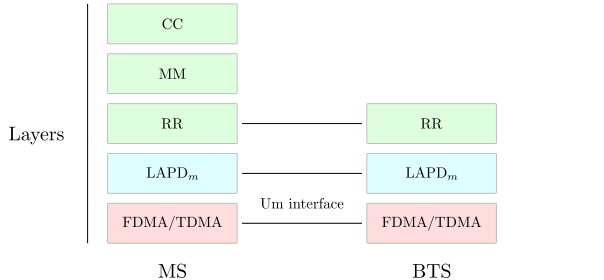
\includegraphics[width=0.75\textwidth]{figures/protocol_stack}
  \caption{The \gls{GSM} protocol stack of the mobile device and the
    \gls{BTS}.\ Data works it way up towards the CC layer from
    the physical FDMA/TDMA layer, through the LAPD$_m$
    data link layer, RR management and MM network
    layers~\cite[p. 108]{gsmnetworks}.}
  \label{fig:protocol_stack}
\end{figure}
The network layers manage individual procedures when it comes to
establishment, maintenance and releasement of radio resources, support
for mobility and identity and establishment, clearing and information
exchanging of call state procedures~\cite[p. 37--38, 91--92,
  176]{layer32}. These network protocols are described more in detail
in \cref{sec:network_layer} and details of \gls{LAPDm} is presented
next.

\subsection{Link Access Protocol, Dm channel}
\gls{LAPDm} ensures sequential order of frames across data link
connections and provides flow control of such frames. It also
detects errors in frames and notifies these to the network layer
entity which it recognizes from the frame type.

\gls{LAPDm} exchanges conform to six different types of formats:
\begin{itemize}
\item \textit{Format A}: the A-format is used for frames without an
  information field and it is sent on \glspl{DCCH}, similar to the
  following formats;
\item \textit{Format B/Bter/B4}: data dedicated to a single user uses
  the B-format for its frame and it is used for actual signalling
  data. Bter and B4 are used for unacknowledged data transmission.
\item \textit{Format Bbis}: a frame in the Bbis-format is used on
  \gls{BCCH}, \gls{PCH}, and \gls{AGCH}.\ It has no address
  information since the sent information is broadcast to all mobile
  devices in which case these are referred to as \glspl{CCCH}.
\item \textit{Format C}: A sixth C-format exists and it is used for
  transmission of random access signals~\cite[p. 9--12]{layer2}.
\end{itemize}

\subsubsection{Frame structure}
The \gls{LAPDm} frame formats consists of an address-, control- and
length indicator field except for the Bbis-format which only carries
network layer information. The B-format also includes an information
field used by third layer protocols. Both the B- and A-format come
with extra fill bits indicated by the length field as seen on
\cref{fig:lapdm_frame}.

\begin{figure}[H]
  \centering
  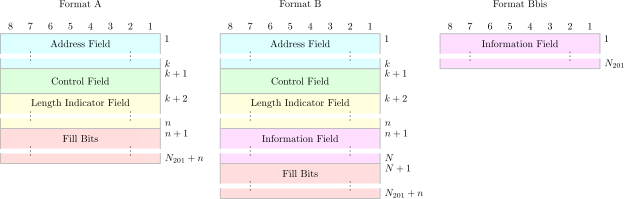
\includegraphics[width=\textwidth]{figures/lapdm}
  \caption{Three examples of LAPDm frame formats consisting of a number of
    fields with varying size of $k$, $n$ and $N$ octets, up to a
    channel specific size parameter, $N_{201}$.}
  \label{fig:lapdm_frame}
\end{figure}

Each field, if present, works as described in the
following~\cite{layer2}:
\begin{itemize}
\item {Address field}: The address field consists of an \gls{EA}, bit,
  a \gls{CR}, bit, a \gls{SAPI}, field and a \gls{LPD}.\ The \gls{EA}
  bit determines if the address field is extended to one more octet
  which may hold additional address info.

  The \gls{CR} bit tells the recipient whether the data is a command
  or a response seen from the \gls{BTS}'s perspective. Data sent from
  the mobile device use the inverted value to inform if it's a command
  or a response.

  The \gls{SAPI} field is used to determine the service of the payload
  such as \gls{RR}, \gls{MM}, \gls{CC} or even \gls{SMS} data.

  The \gls{LPD} field is reserved and should not be set.

\item {Control field}: This field conform to three different formats,
  the \textit{information transfer}, I-format, the
  \textit{supervisory}, S-format and the \textit{unnumbered},
  U-format. They control which action to take based on the \gls{CR}
  bit from the address field such as acknowledge or unacknowledge
  certain received information and even request retransmission of
  information. The S-format supervises and is used to control the next
  move such as acknowledge an I-frame, request retransmission etc.,
  while the I-format is used to transfer information between network
  layer entities. The U-format may be used to provide additional
  control functions.

\item {Information field}: this field is the payload of the network
  layer protocols and is not processed.
\end{itemize}
\subsection{Network layer}
\label{sec:network_layer}
The third layer consists of three different protocols for network
management and these are individually identified by a \gls{PD}, and
their transaction origin by a \gls{TI}, value. The frame format is
mostly identical for all three protocols and they all contain the
identification, message type and the parameters assigned to that
specific message type.

Apart from origin, the \gls{TI} value also distinguishes messages
within a transaction, however only the \gls{CC} protocol allow several
simultaneously transactions. The mobile device and the \gls{NSS} may
use the same \gls{TI} values set by the three least significant bits
since their origin differ and the \gls{TI}'s most significant bit
identifies the origin~\cite[p. 87]{layer3}.
\subsubsection{Radio resource management}
\label{sec:rr}
Procedures of radio resource management are necessary to establish,
maintain and release \gls{RR} data link connections between the mobile
device and the network. These common transmission resources are partly
managed and processed on both ends on the Um interface, but also
further in the network e.g.\ at the \gls{MSC}.\ This allows further
procedures like cell selection and handover procedures.

Radio resource management is assigned the \gls{PD},
$06$~\cite[p. 107]{gsmnetworks}.

The \gls{RR} procedures manage the logical and physical channels which
are then processed in the remaining network layer
protocols~\cite[p. 37--38]{layer32}.

\subsubsection{Mobility management}
\label{sec:mm}

Unlike \gls{RR} management, generally, neither \gls{MM} nor \gls{CC},
with a few exceptions, are involved at the \gls{BTS} and both of these
protocols are managed by the \gls{NSS} and the mobile device. This allows
transparent information exchange on logical channels provided by the
\gls{RR} protocol.

The functions of mobility management procedures are mainly location
area updates and providing user identity
confidentiality~\cite[p. 91]{layer32}.

Mobility management is assigned the \gls{PD},
$05$~\cite[p. 107]{gsmnetworks}.
\subsubsection{Call control}
\label{sec:cc}

The \gls{CC} protocol is an application that consists of entities that make
large communicating finite state machines which controls functions
such as call establishment procedures, call clearing procedures and
call information phase procedures etc.~\cite[p. 176]{layer32}.

Call control and supplementary services are assigned the \gls{PD},
$03$~\cite[p. 107]{gsmnetworks}.